% Thesis Chapter 2 — Profile-driven simulation framework
% Seeded from manuscript methodology (§3) and internal framework code.
% Thesis-level emphasis: the framework itself as a reusable research instrument,
% not merely an implementation detail of the NC experiments.
%
% Figures reused from manuscript package (paths relative to paper/thesis/):
%   ../latex_gpt/figures/fig1_system_architecture.pdf
%   ../latex_gpt/figures/fig2_weight_mapping.pdf
%   ../latex_gpt/figures/figS2_nonideality.png
%   ../latex_gpt/figures/fig6_physical_compensation.pdf
%   ../latex_gpt/figures/fig7_retention_curve.pdf
%   ../latex_gpt/figures/fig_nl_gradient_distortion.pdf
%   ../latex_gpt/figures/fig11_energy_breakdown.pdf
%
% Cross-references:
%   Chapter 1 (\ref{chap:hat-instance-overfitting}) — HAT and instance overfitting
%   Chapter 3 (\ref{chap:severe-nl}) — severe nonlinearity boundary
%   Manuscript: \citep{...} for device literature, \ref{sec:methodology} for methodology

\chapter{Profile-driven simulation framework}
\label{chap:framework}

\section{Introduction: why profile-driven simulation}

Organic optoelectronic compute-in-memory systems are usually judged by device-level figures of merit: conductance window, retention time, write asymmetry, and optical responsivity. Those metrics are necessary, but they are not sufficient to answer the system question that matters for deployment. What accuracy survives once a modern vision backbone is mapped to an analog array with structured mismatch, finite readout precision, and a sub-linear photoresponse? Answering that question requires a deliberate bridge between the measurement laboratory and the algorithm training loop.

This chapter describes the simulation framework that provides that bridge. The design principle is \emph{profile-driven}: every physically relevant assumption enters through a single structured configuration object, so that a literature-derived prior and an in-house measured profile are interchangeable inputs to the same training or evaluation script. This is important because early device characterization rarely arrives as a single ``device score.'' Instead, it is distributed across several measurement modalities—multilevel programming, repeated same-state reads, cross-device statistics, retention fitting, and photoresponse characterization. The framework treats these measurements as structured calibration inputs rather than as informal narrative context.

The thesis therefore treats the framework itself as a research instrument, not merely as an implementation detail of the manuscript experiments. Its contributions are threefold. First, a set of pluggable physical interfaces that let device parameters enter the forward path without changing model architecture code. Second, a deep integration with PyTorch autograd that makes hardware-aware training a drop-in training-mode switch rather than a custom optimizer rewrite. Third, an external validation against the CrossSim crossbar simulator that confirms numerical consistency in a shared operating regime and highlights where organic-specific extensions diverge from generic RRAM models.

\section{Pluggable physical interfaces}
\label{sec:pluggable-interfaces}

The central design decision is to encapsulate every physical effect in a single replaceable profile object, then apply that profile uniformly across all analog-mapped layers. This section walks through the five physical interfaces: the device model, mismatch variability, nonlinear write asymmetry, retention drift, and the optoelectronic front end.

\subsection{The device profile as a structured configuration object}

At the core of the framework is a configuration dataclass that collects all parameters needed to simulate an analog crossbar layer. A profile instance specifies the conductance window $[G_{\min}, G_{\max}]$, the number of discrete conductance states $n_{\text{states}}$, the variability coefficients $(\sigma_{\text{C2C}}, \sigma_{\text{D2D}})$, the retention time constants $(\tau_1, \tau_2, A_0)$, the photoresponse nonlinearity $\gamma_{\text{phys}}$, and the write-asymmetry exponents $(\mathrm{NL}_{\mathrm{LTP}}, \mathrm{NL}_{\mathrm{LTD}})$. Table~\ref{tab:measurement-mapping} (reproduced from the manuscript) shows the direct mapping between laboratory characterization procedures and simulator fields.

\begin{table}[htbp]
\centering
\caption{Measurement-to-simulator parameter mapping. A literature-derived profile and an in-house measured profile populate the same fields and therefore drive the same training scripts.}
\label{tab:measurement-mapping}
\begin{tabular}{lll}
\toprule
\textbf{Measurement} & \textbf{Typical characterization method} & \textbf{Simulator parameter(s)} \\
\midrule
Conductance window & Multilevel programming I--V sweep & \texttt{G\_min}, \texttt{G\_max} \\
Resolvable state count & Programming resolution / histogram separability & \texttt{n\_states} \\
Cycle-to-cycle variability & Repeated read/program at fixed target state & \texttt{sigma\_c2c} \\
Device-to-device mismatch & Cross-device or cross-array statistics & \texttt{sigma\_d2d} \\
Retention dynamics & Time-decay curve fit & \texttt{A\_0}, \texttt{tau\_1}, \texttt{tau\_2} \\
Photoresponse nonlinearity & $I_{\text{photo}}$ vs intensity & \texttt{gamma\_phys} \\
\bottomrule
\end{tabular}
\end{table}

The profile object is passed to every analog layer at construction time. Because the layer code contains no hard-coded physics, switching from a literature prior to a measured device recalibration requires only replacing the profile instance; no model definition or training script changes. This is the sense in which the framework is profile-driven. It also means that the experiments reported in later chapters of this thesis are, in principle, fully reproducible on new device data once the corresponding profile is populated.

\subsection{Device variability: D2D and C2C}
\label{subsec:d2d-c2c-interface}

The framework models two sources of device variability. Device-to-device (D2D) mismatch is treated as a static perturbation sampled once at initialization:
\begin{equation}
\boldsymbol{\epsilon}_{\text{D2D}} \sim \mathcal{N}\left(0, \sigma_{\text{D2D}}^{2} \Delta G^{2}\right), \qquad \Delta G = G_{\max} - G_{\min}.
\label{eq:d2d-model}
\end{equation}
This perturbation is stored as a persistent buffer and is applied to every subsequent forward pass. It captures fixed manufacturing mismatch across programmed devices on the array. Cycle-to-cycle (C2C) variation is modeled as a zero-mean Gaussian perturbation resampled on each forward pass:
\begin{equation}
\boldsymbol{\epsilon}_{\text{C2C}}^{(t)} \sim \mathcal{N}\left(0, \sigma_{\text{C2C}}^{2} \Delta G^{2}\right).
\label{eq:c2c-model}
\end{equation}
The noisy effective weight becomes
\begin{equation}
\widehat{\mathbf{W}}^{(t)} = \left(\widetilde{\mathbf{G}}^{+} - \widetilde{\mathbf{G}}^{-}\right) + \boldsymbol{\epsilon}_{\text{D2D}} + \boldsymbol{\epsilon}_{\text{C2C}}^{(t)},
\label{eq:noisy-weight}
\end{equation}
with the C2C term disabled when the experiment calls for clean or D2D-only evaluation. Both variances are applied in the conductance domain so that noise magnitude scales with the physical dynamic range, a choice that preserves interpretability when the conductance window changes between device generations.

In addition to the canonical uniform-noise mode, the framework supports a proportional-noise mode where the noise magnitude scales with the instantaneous conductance state:
\begin{equation}
\boldsymbol{\epsilon}^{(t)}_{\text{prop}} \sim \mathcal{N}\left(0, \sigma^2 \lvert \mathbf{G}_{\text{current}} \rvert^2\right).
\label{eq:proportional-noise}
\end{equation}
This mode is useful for stress-testing the robustness of trained models under more physically realistic noise distributions, and it is accessed by changing a single string field in the profile object.

\subsection{Nonlinear write asymmetry}
\label{subsec:nl-interface}

Nonlinear programming is implemented not as a pulse-accurate write simulator but as a first-order behavioral proxy that modulates the straight-through estimator backward pass according to the current conductance position. If a weight update would increase conductance, the surrogate gradient is scaled as
\begin{equation}
\frac{\partial \mathcal{L}}{\partial G}\Big|_{\mathrm{LTP}} \propto \left(\frac{G_{\max}-G}{G_{\max}-G_{\min}}\right)^{\mathrm{NL}_{\mathrm{LTP}}-1},
\label{eq:nl-ltp}
\end{equation}
whereas a conductance-decreasing update is scaled as
\begin{equation}
\frac{\partial \mathcal{L}}{\partial G}\Big|_{\mathrm{LTD}} \propto \left(\frac{G-G_{\min}}{G_{\max}-G_{\min}}\right)^{|\mathrm{NL}_{\mathrm{LTD}}|-1}.
\label{eq:nl-ltd}
\end{equation}
When $\mathrm{NL}_{\mathrm{LTP}} = 1$ and $\mathrm{NL}_{\mathrm{LTD}} = -1$, the model reduces to the identity STE used in the nominal experiments. Larger magnitudes increase the dependence of the update on the current conductance position: potentiation becomes weaker near $G_{\max}$ and depression becomes weaker near $G_{\min}$.

It is important to emphasize the abstraction level. The $NL=2.0$ boundary identified in Chapter~\ref{chap:failure-mode-atlas} reflects the limit of this first-order gradient-scaling approximation under a severe matched stress setting, not a universal impossibility theorem for all organic write processes. Its practical purpose is to ensure that measured nonlinearity coefficients can enter the optimization path through the same profile interface used by inference-only experiments.

\subsection{Retention decay}
\label{subsec:retention-interface}

Post-programming weight drift is modeled with a double-exponential retention law. For a programmed conductance $G$ and elapsed inference time $t$, the decayed conductance is
\begin{equation}
G(t) = G_{\min} + \left(G - G_{\min}\right) \left[A_1 \exp\left(-t/\tau_1\right) + A_2 \exp\left(-t/\tau_2\right) + A_0\right],
\label{eq:retention}
\end{equation}
with $A_1 = A_2 = (1-A_0)/2$ and $A_0 = 0.6$. The default parameters are $\tau_1 = 140$~ms and $\tau_2 = 610$~ms, taken from the handbook's device prior based on DNTT retention measurements \citep{vincze2026dualplasticity}. This form captures an initial fast drop, an intermediate slower decay, and a non-zero persistent fraction.

Retention is applied after conductance quantization and before the stochastic noise terms in the analog forward model. This ordering reflects the interpretation that weights are first programmed to discrete conductance levels, then drift in time, and are finally observed under fixed mismatch and read-time variability. The framework additionally supports a state-dependent retention extension where high-conductance states decay faster, allowing stress-testing of long-term stability under realistic relaxation dynamics.

\begin{figure}[t]
    \centering
    \includegraphics[width=0.78\linewidth]{../latex_gpt/figures/fig7_retention_curve}
    \caption{Double-exponential retention decay reproduced from the manuscript. The curve shows the programmed conductance fraction remaining as a function of elapsed time, with the fast ($\tau_1=140$~ms) and slow ($\tau_2=610$~ms) components visible.}
    \label{fig:retention-curve}
\end{figure}

\subsection{Optoelectronic front-end compensation}
\label{subsec:frontend-interface}

To model the organic phototransistor front end, the framework uses a sub-linear photocurrent response
\begin{equation}
I_{\text{photo}} = \alpha P^{\gamma_{\text{phys}}} + I_{\text{dark}} + \eta_{\text{shot}},
\label{eq:photocurrent}
\end{equation}
where $P$ denotes the incident optical signal, $\alpha$ is a responsivity scale, $\gamma_{\text{phys}}$ captures the non-linear transfer characteristic, $I_{\text{dark}}$ is dark current, and $\eta_{\text{shot}}$ is a signal-dependent stochastic term. The compensation mechanism applies an inverse-gamma preprocessing step
\begin{equation}
P_{\text{in}} = X^{1/\gamma_{\text{phys}}},
\label{eq:inverse-gamma}
\end{equation}
so that the subsequent device response becomes approximately linear in the original normalized input $X$.

This compensation is not treated as a universally beneficial transformation. Because shot-noise variance scales with photocurrent, inverse-gamma preprocessing also reshapes the noise statistics. The benefit must therefore be interpreted as a task- and regime-dependent trade-off rather than as a free robustness improvement. In the current workflow, the front-end is used explicitly in the physical-compensation experiments and analyzed separately from the weight-noise robustness experiments so that frontend compensation and hardware-aware training are not conflated.

\begin{figure}[t]
    \centering
    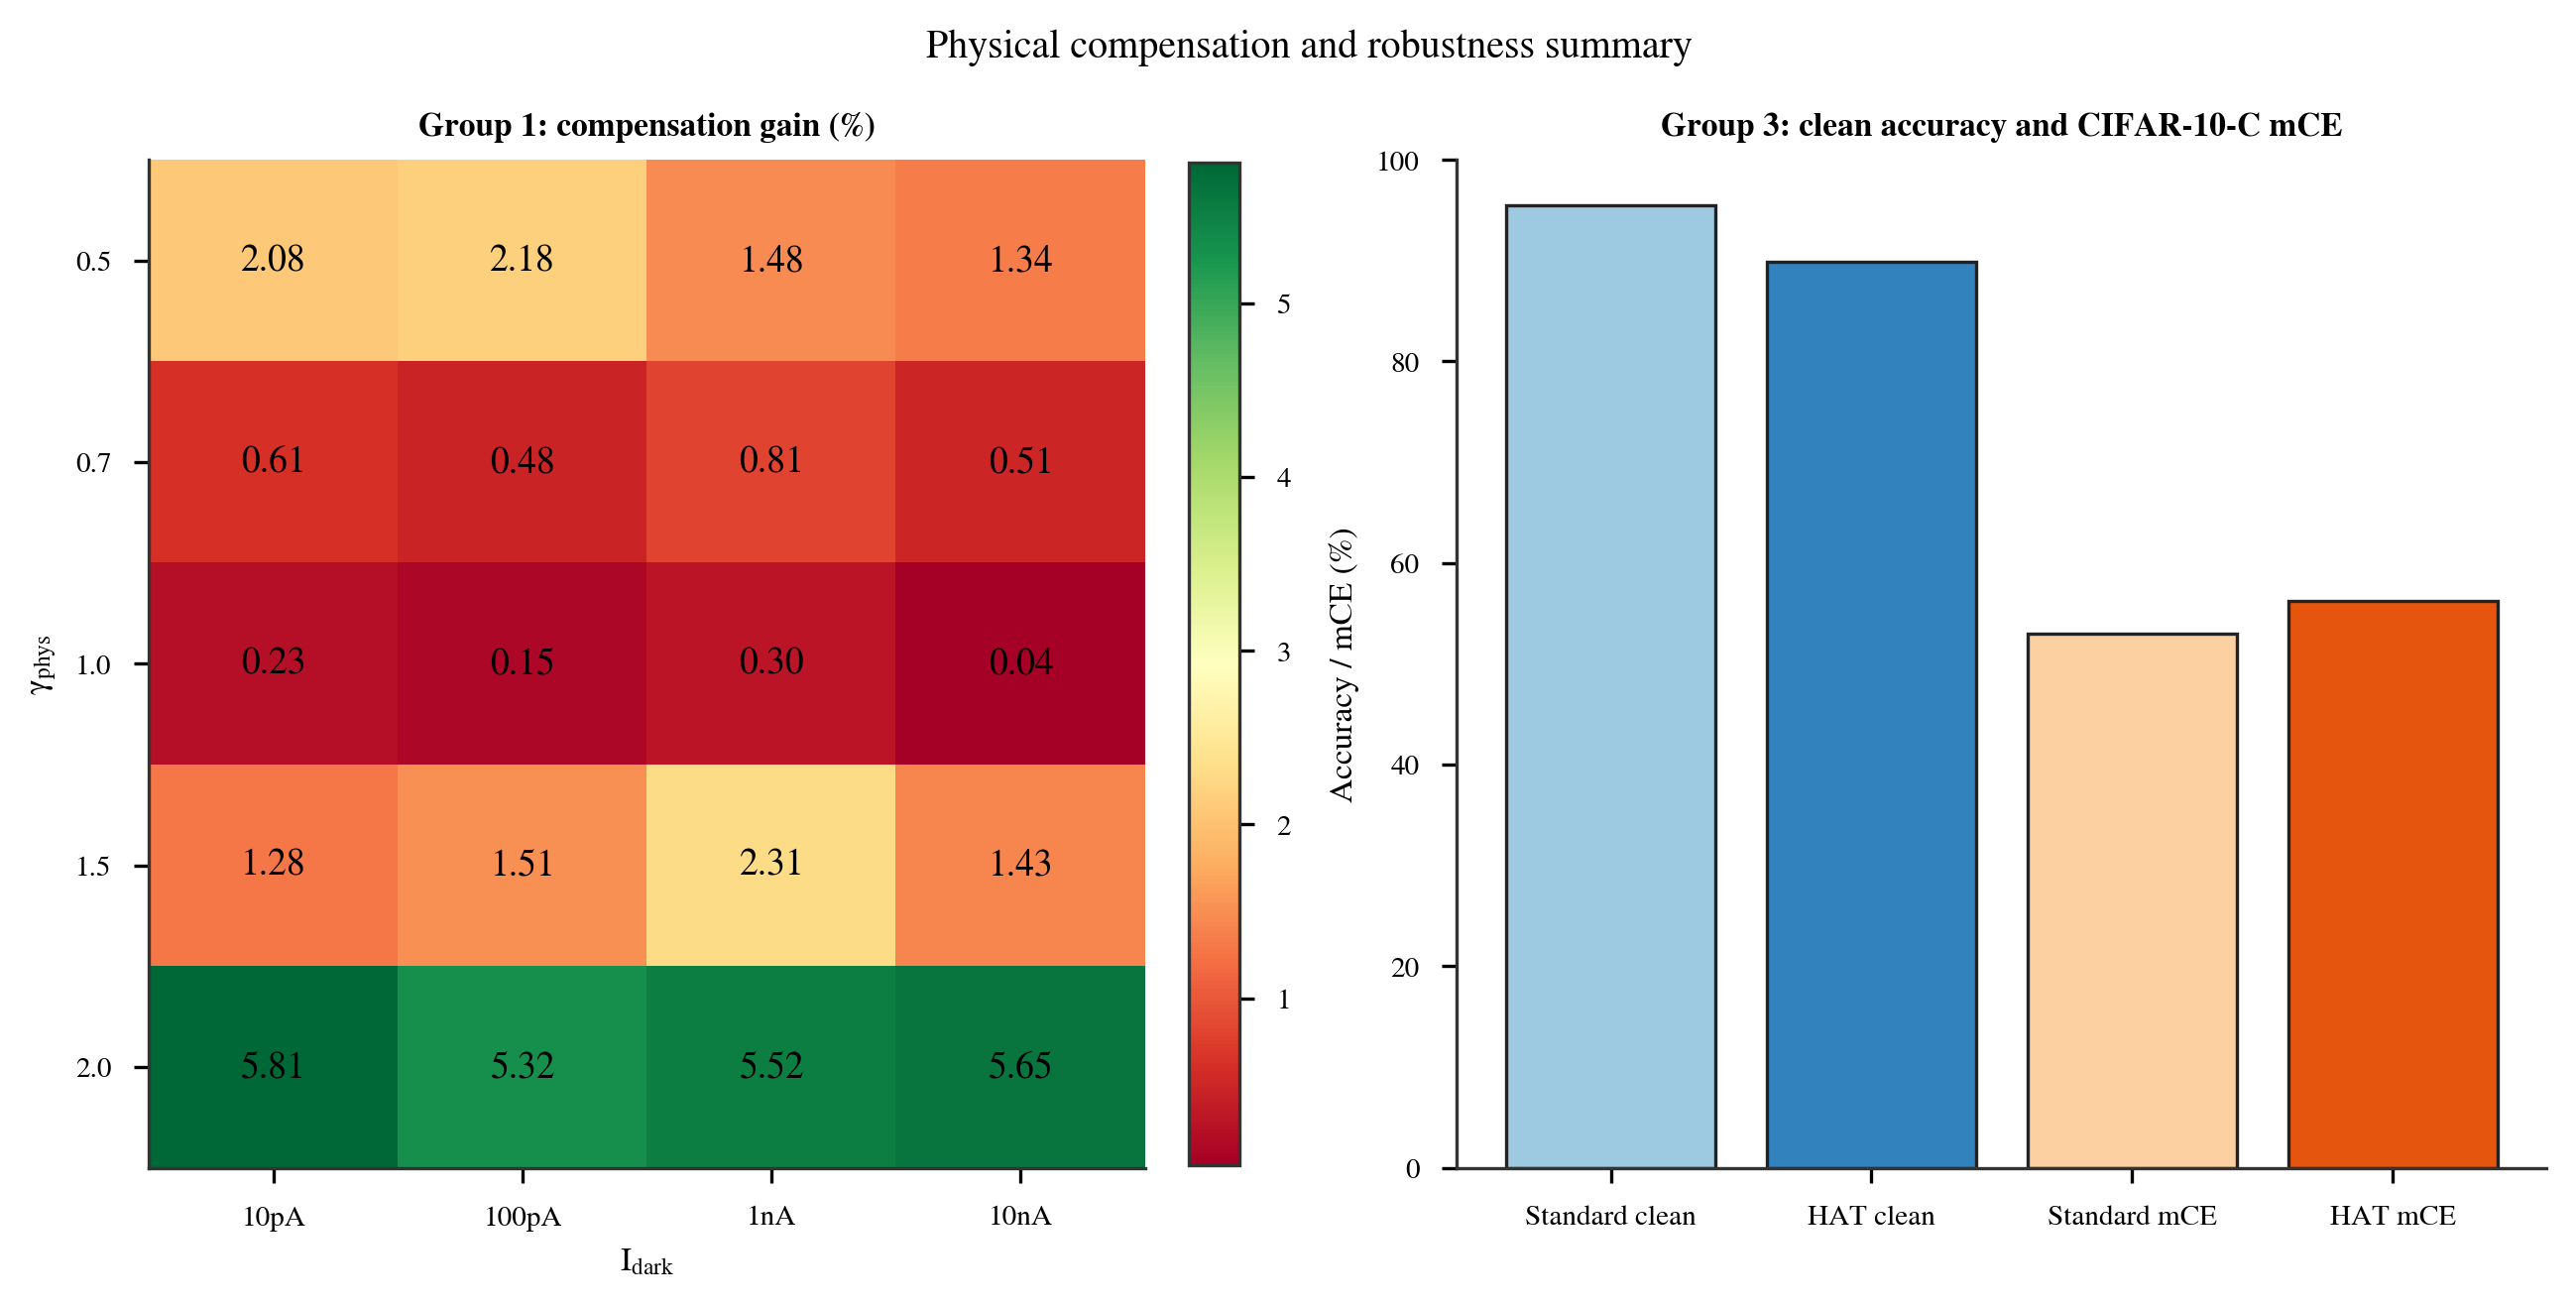
\includegraphics[width=0.78\linewidth]{../latex_gpt/figures/fig6_physical_compensation}
    \caption{Physical front-end compensation reproduced from the manuscript. The inverse-gamma preprocessor linearizes the sub-linear photoresponse, but also reshapes shot-noise variance.}
    \label{fig:frontend-compensation}
\end{figure}

\subsection{ADC quantization and peripheral non-ideality}

At the output of each crossbar column, an analog-to-digital converter discretizes the accumulated current. The framework models ADC non-idealities separately from the energy counts. For a $b$-bit converter, the continuous current is first quantized to $2^b$ nominal codes, and differential non-linearity (DNL) is injected by perturbing each step width:
\begin{equation}
\Delta_{\text{actual}}[i] = \Delta_{\text{ideal}} \left(1 + \mathcal{N}(0, \sigma_{\text{DNL}}^2)\right),
\label{eq:dnl}
\end{equation}
with $\sigma_{\text{DNL}} = 0.5$~LSB in the default configuration. This perturbation is instantiated as a fixed per-ADC offset table, so the converter behaves analogously to a static D2D imperfection rather than fresh C2C noise.

The energy model is kept explicitly separate from the accuracy model. A first-order estimate sums analog MAC cost, ADC cost, DAC cost, digital MAC cost, and memory-access cost:
\begin{equation}
E_{\text{total}} = E_{\text{analog}} + E_{\text{ADC}} + E_{\text{DAC}} + E_{\text{digital}} + E_{\text{buffer}}.
\label{eq:energy-total}
\end{equation}
This separation is deliberate: it allows measured accuracy and estimated energy to be combined in a Pareto analysis without conflating the physical fidelity of the forward simulator with the placeholder nature of the energy constants.

\section{PyTorch autograd integration}
\label{sec:pytorch-integration}

The framework is implemented as a collection of drop-in PyTorch modules that replace standard \texttt{nn.Linear} and \texttt{nn.Conv2d} layers with analog-aware equivalents. This section explains how the physical pipeline is integrated into the autograd graph, making hardware-aware training a training-mode switch rather than a custom training loop rewrite.

\subsection{Straight-through estimator quantizer}

The fundamental autograd primitive is a custom \texttt{torch.autograd.Function} that implements uniform quantization with an identity backward pass. In the forward direction, the input is clamped to $[x_{\min}, x_{\max}]$, normalized to $[0,1]$, rounded to the nearest of $n_{\text{levels}}$ discrete values, and denormalized back:
\begin{equation}
x_{\text{quant}} = \left\lfloor \frac{x_{\text{clamped}} - x_{\min}}{x_{\max} - x_{\min}} (n_{\text{levels}} - 1) \right\rceil \frac{x_{\max} - x_{\min}}{n_{\text{levels}} - 1} + x_{\min}.
\label{eq:ste-forward}
\end{equation}
In the backward direction, gradients pass straight through unchanged: $\partial \mathcal{L} / \partial x_{\text{quant}}$ is returned as $\partial \mathcal{L} / \partial x$. This is the standard straight-through estimator (STE) approximation for piecewise-constant conductance states.

What distinguishes this implementation is that the backward pass optionally rescales the gradient by the nonlinear write asymmetry factors defined in Equations~(\ref{eq:nl-ltp})--(\ref{eq:nl-ltd}). The quantizer therefore serves two purposes simultaneously: it enables gradient flow through discrete conductance levels, and it injects measured write nonlinearity into the optimizer through the same code path.

\subsection{Differential-pair conductance mapping}

Each analog-mapped weight tensor $\mathbf{W}$ is converted into a differential-pair conductance representation. Let
\begin{equation}
\mathbf{W}^{+} = \max(\mathbf{W}, 0), \qquad
\mathbf{W}^{-} = \max(-\mathbf{W}, 0).
\label{eq:weight-split}
\end{equation}
To avoid propagating gradients through the normalization constant, the scale factor is detached from the computation graph:
\begin{equation}
s_W = \lVert \mathbf{W} \rVert_{\infty}^{\mathrm{detach}} + \varepsilon.
\label{eq:scale-detach}
\end{equation}
The positive and negative components are then mapped to the physical conductance range $[G_{\min}, G_{\max}]$:
\begin{equation}
\mathbf{G}^{+} = G_{\min} + \frac{\mathbf{W}^{+}}{s_W}(G_{\max} - G_{\min}), \qquad
\mathbf{G}^{-} = G_{\min} + \frac{\mathbf{W}^{-}}{s_W}(G_{\max} - G_{\min}).
\label{eq:conductance-mapping}
\end{equation}
The programmed conductances are quantized to $n_{\text{states}}$ discrete levels with the STE:
\begin{equation}
\widetilde{\mathbf{G}} = \operatorname{STEQuantize}(\mathbf{G}; n_{\text{states}}, G_{\min}, G_{\max}),
\label{eq:ste-quantize}
\end{equation}
so that the forward path observes discrete conductance states while the backward path passes gradients as identity.

The effective analog weight used for vector-matrix multiplication is the differential conductance
\begin{equation}
\mathbf{W}_{\text{eff}} = \widetilde{\mathbf{G}}^{+} - \widetilde{\mathbf{G}}^{-},
\label{eq:eff-weight}
\end{equation}
optionally followed by scale recovery:
\begin{equation}
\widehat{\mathbf{W}}_{\text{eff}} = \mathbf{W}_{\text{eff}} \cdot \frac{\lVert \mathbf{W} \rVert_{\infty}^{\mathrm{detach}}}{G_{\max} - G_{\min}}.
\label{eq:scale-recovery}
\end{equation}

\begin{figure}[t]
    \centering
    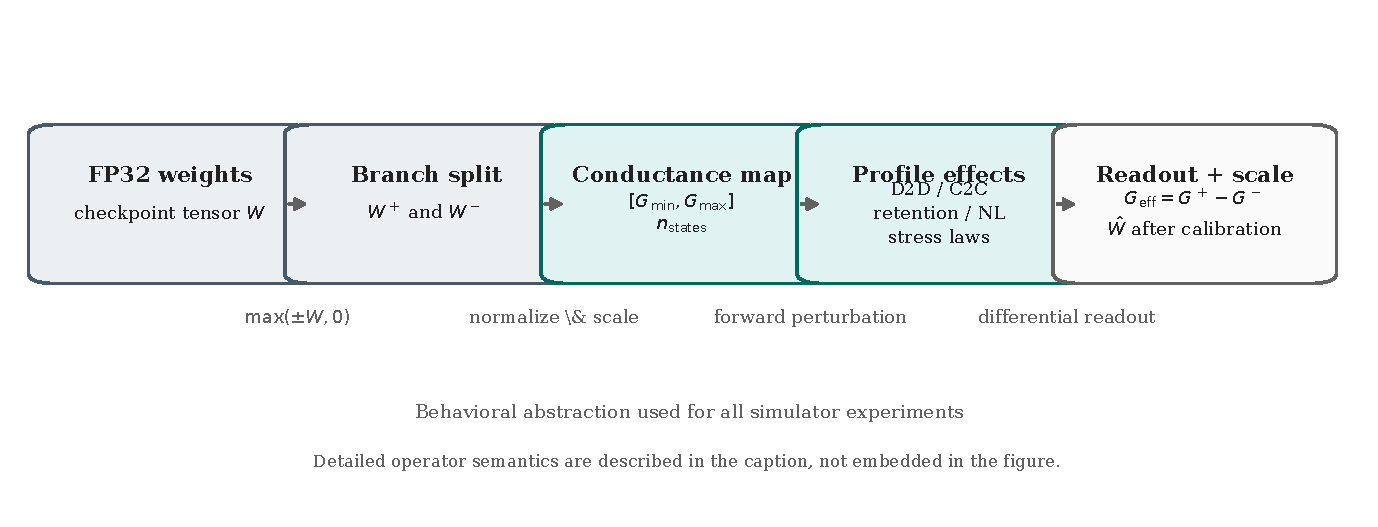
\includegraphics[width=0.85\linewidth]{../latex_gpt/figures/fig2_weight_mapping}
    \caption{Differential-pair weight-to-conductance mapping reused from the manuscript. The digital weight tensor is split into positive and negative parts, normalized, mapped to the conductance window, quantized, and recombined as a differential effective weight.}
    \label{fig:weight-mapping}
\end{figure}

Scale recovery is one of the key physical simplifications of the present work. It is implemented as an ideal post-array digital rescaling step using layer-wise floating-point factors. That is a useful first-order behavioral abstraction for algorithm-device co-design, but it implicitly assumes that the peripheral readout chain can realize the required gain calibration with negligible quantization or control overhead. In this thesis, scale recovery is therefore treated as a calibrated digital post-processing primitive rather than as a claim of zero-cost physical circuitry.

\subsection{Forward-path noise injection}

The analog layer forward pass follows a strict physical ordering:
\begin{enumerate}
\item \textbf{Quantization:} Float weight $\rightarrow$ differential conductance pair $\rightarrow$ STE quantization.
\item \textbf{Retention:} Optional double-exponential decay applied to programmed conductances.
\item \textbf{Mismatch:} D2D noise (fixed buffer) and C2C noise (resampled per forward) added to the effective weight.
\item \textbf{Scale recovery:} Optional digital rescaling to restore the original weight magnitude.
\item \textbf{Linear operation:} Standard \texttt{F.linear} or \texttt{F.conv2d} with the noisy effective weight.
\end{enumerate}

This ordering is not arbitrary. It reflects the physical interpretation that weights are first programmed to discrete conductance levels, then drift in time, and are finally observed under fixed mismatch and read-time variability. Because every step is differentiable via the STE, the entire pipeline participates in gradient descent during hardware-aware training.

\subsection{Backward-path gradient scaling}

When nonlinear write asymmetry is enabled, the STE backward pass is modified to scale gradients by the current conductance position. For a gradient $g = \partial \mathcal{L} / \partial G$, the returned surrogate is
\begin{equation}
g_{\text{surrogate}} = \begin{cases}
g \cdot \left(\dfrac{G_{\max} - G}{G_{\max} - G_{\min}}\right)^{\mathrm{NL}_{\mathrm{LTP}} - 1} & \text{if } g \ge 0, \\[1.2em]
g \cdot \left(\dfrac{G - G_{\min}}{G_{\max} - G_{\min}}\right)^{|\mathrm{NL}_{\mathrm{LTD}}| - 1} & \text{if } g < 0.
\end{cases}
\label{eq:nl-gradient-scaling}
\end{equation}

This scaling has a simple physical interpretation. Near $G_{\max}$, further potentiation is physically difficult; the gradient scaling therefore suppresses updates that would push the conductance beyond the measurable window. Near $G_{\min}$, the same logic applies to depression. The scaling is applied element-wise inside the autograd backward call, so it requires no changes to the optimizer or learning-rate schedule.

\begin{figure}[t]
    \centering
    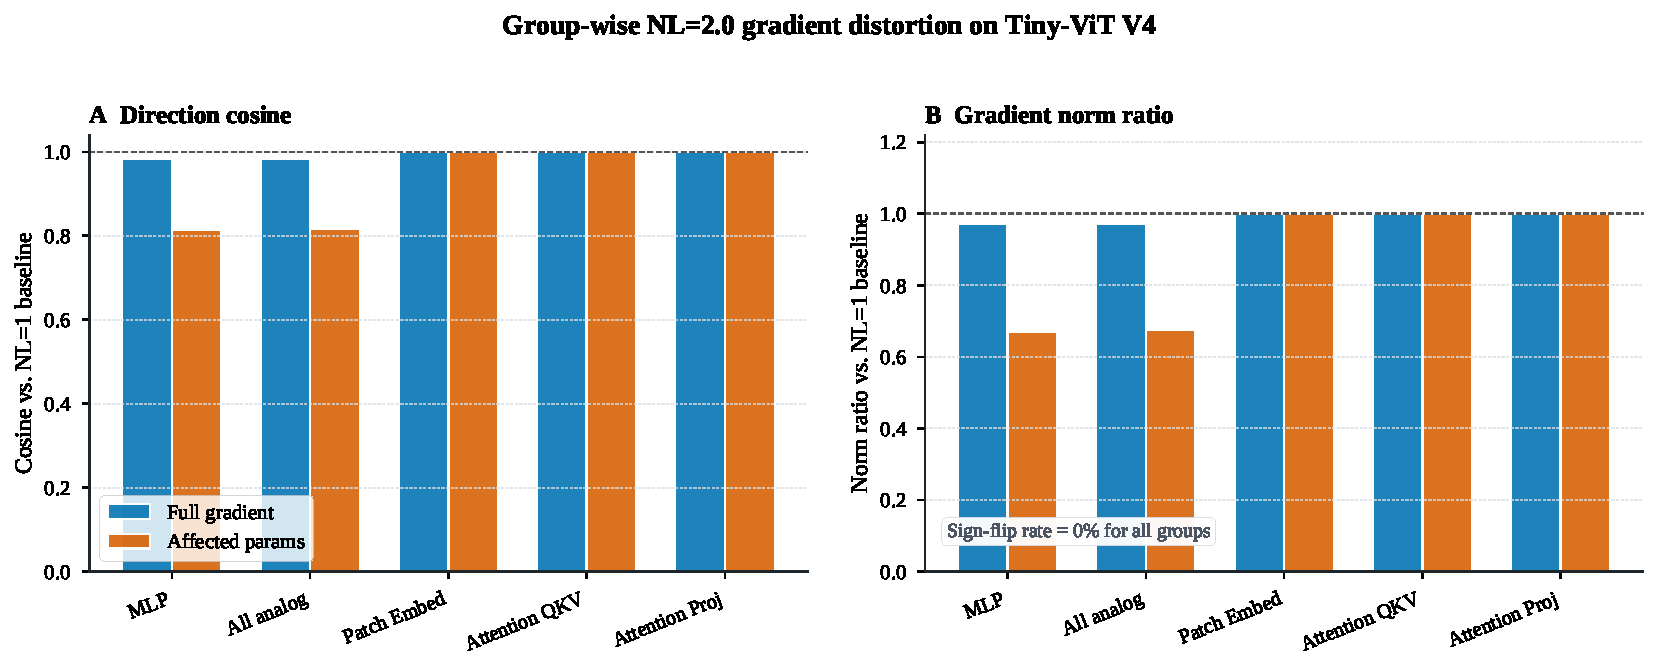
\includegraphics[width=0.78\linewidth]{../latex_gpt/figures/fig_nl_gradient_distortion}
    \caption{Nonlinear gradient distortion reproduced from the manuscript. The plots show how the surrogate gradient is scaled as a function of conductance position for several NL values.}
    \label{fig:nl-gradient}
\end{figure}

It is worth repeating that this is an optimizer-side abstraction rather than a pulse-by-pulse device simulator. The framework does not track individual programming pulses, write-verify iterations, or conductance trajectory history. It instead provides a direct way to inject measured write asymmetry into training-time robustness studies through the same profile interface used for inference-only experiments.

\subsection{Model conversion and layer replacement}

The framework provides a model conversion utility that performs in-place replacement of PyTorch layers. Given a standard model (e.g., Tiny-ViT from \texttt{timm}), the utility traverses the module tree and substitutes analog equivalents for layers whose names match a set of configurable patterns. For Tiny-ViT, the analog-mapped layers are the patch-embedding convolutions, the attention projection matrices $\mathbf{W}_Q$, $\mathbf{W}_K$, $\mathbf{W}_V$, the attention output projection, and the two feed-forward matrices in each transformer block. Mobile inverted bottleneck convolution (MBConv) blocks, downsampling paths, local depthwise convolutions, dynamic attention products, softmax, LayerNorm, activation functions, and the classification head remain digital.

This split is motivated by array utilization. Dense operators map naturally to crossbars because their weight tensors can be flattened into large matrix tiles with high occupancy. Depthwise convolutions and dynamic attention products either have poor output-unit utilization or require input-dependent matrices that cannot be pre-programmed into non-volatile arrays. The same split is also consistent with the current organic-optoelectronic hardware literature, which already demonstrates regular static array programming and readout much more naturally than fully dynamic token-token interaction engines.

\begin{figure}[t]
    \centering
    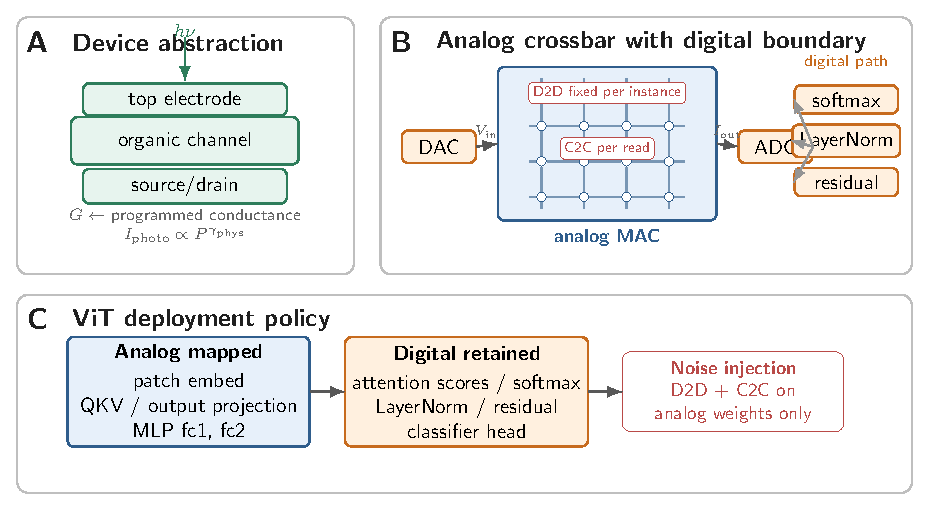
\includegraphics[width=0.88\linewidth]{../latex_gpt/figures/fig1_system_architecture}
    \caption{Hybrid system architecture reused from the manuscript. Dense linear operators execute on differential-pair crossbar arrays, while control-heavy or utilization-poor operators remain on a digital coprocessor.}
    \label{fig:system-arch}
\end{figure}

For Tiny-ViT-5M, the mapping sends $4{,}730{,}016$ parameters to the analog domain and leaves $662{,}748$ parameters digital, corresponding to an analog-mapped parameter ratio of $87.7\,\%$. Under a $128 \times 128$ physical array constraint and differential-pair storage, this requires 812 arrays and $13{,}303{,}808$ individual devices. The analog footprint is concentrated in the transformer stages: patch embedding contributes only 8 differential-pair arrays, Stage 1 contributes 48 arrays, Stage 2 contributes 384 arrays, and Stage 3 contributes 372 arrays.

The conversion utility copies learned weights from the original digital layers into the analog replacements, so a pre-trained checkpoint can be converted to hybrid form without re-initialization. This is essential for the fine-tuning experiments reported in later chapters, where Tiny-ViT is loaded from an ImageNet-pretrained checkpoint and then adapted to analog deployment.

\section{CrossSim sanity-check validation}
\label{sec:crosssim-validation}

A simulation framework is only as credible as its validation against independent tools. This section describes a cross-framework comparison against CrossSim, a GPU-accelerated crossbar-accuracy workflow with parasitic resistance, ADC, drift, and lookup-table-based training models \citep{crosssim2026}.

\subsection{Shared-regime experimental protocol}

Because CrossSim was developed primarily around inorganic resistive memories, it does not directly expose inverse-gamma optoelectronic photoresponse or organic-specific double-exponential retention as first-class device primitives. A direct comparison is therefore limited to the \emph{shared regime}: 8-bit ADC, uniform noise, deterministic baseline, and standard differential-pair mapping. Both frameworks were configured to use positive-only inputs, calibrated ADC ranges, and comparable conductance windows.

The comparison was performed on a deterministic 1\,000-image CIFAR-10 test subset. This subset protocol was chosen because of CrossSim throughput constraints on the full test set. The protocol is disclosed explicitly; the results should be read as a sanity check rather than as a comprehensive benchmark.

\subsection{Results and interpretation}

In the clean baseline regime, the two frameworks produced consistent inference accuracy: $86.2\,\%$ (ours) versus $83.7\,\%$ (CrossSim) at 8-bit ADC on the shared subset. Under uniform noise injection at $\sigma=5\,\%$, however, the predictions diverged substantially: $81.63\pm0.56\,\%$ (ours) versus $67.20\pm2.67\,\%$ (CrossSim), a qualitative gap of $14.43$~percentage points.

This divergence is informative rather than alarming. It highlights that accuracy predictions are highly sensitive to the exact noise-to-conductance mapping: how variances are referenced (global window versus local state), whether noise is added before or after quantization, and how differential-pair common-mode cancellation is modeled. These are precisely the details that a profile-driven framework makes explicit. The CrossSim comparison therefore serves as a valuable sanity check on the baseline implementation while confirming that the organic-specific extensions—photoresponse, retention, proportional noise, and ensemble resampling—represent genuine capability additions beyond the shared inorganic toolset.

The frameworks are best viewed as complementary. CrossSim provides Simulation Program with Integrated Circuit Emphasis (SPICE)--calibrated parasitic models and detailed peripheral circuits for inorganic arrays. The present framework provides a lightweight, PyTorch-native stack for organic-device profile substitution, end-to-end hardware-aware training, and rapid algorithm-device co-design. Neither replaces the other; together they bracket the space of simulation fidelity versus experimental agility.

\section{Limitations of the first-order behavioral model}

While the framework provides a robust bridge between device parameters and system accuracy, it is fundamentally a first-order behavioral simulation framework. Several complex physical realities are abstracted, and these limitations should be kept in mind when interpreting the results of later chapters.

First, the digital overhead of scale masking is modeled as an exact floating-point operation. In physical hardware, layer-wise rescaling would require either high-precision digital multipliers or finely programmable transimpedance-amplifier gains, which introduce hidden energy and area overheads not fully penalized in the current energy model.

Second, position-dependent IR drop along crossbar wordlines and bitlines, as well as sneak-path currents in passive arrays, are not modeled in the current framework. These effects introduce systematic, input-pattern-dependent weight distortion that is distinct from the stochastic variability captured by the C2C and D2D terms. The framework includes scalar placeholders for these effects, but they are not geometry-aware.

Third, the energy parameters are anchored to 28~nm handbook assumptions and should be interpreted as first-order system-model estimates rather than final silicon measurements. Array-to-digital interconnect energy is absorbed into SRAM read/write cost terms, and dedicated routing overhead is not separately itemized.

Finally, the framework assumes ideal single-shot programming and therefore excludes iterative write-verify overhead for 4-bit conductance states. Extending the framework toward measured level tables and explicit integral non-linearity remains future work.

\section{Summary and transition}

This chapter has described the profile-driven simulation framework that underpins the experimental contributions of this thesis. The key design principles are:
\begin{itemize}
\item \textbf{Profile-driven parameterization:} All physical effects enter through a single structured configuration object, making literature priors and measured profiles interchangeable.
\item \textbf{Pluggable physical interfaces:} Device variability, nonlinear write asymmetry, retention drift, optoelectronic front-end distortion, and ADC non-ideality are modular extensions that can be enabled or disabled without changing model architecture code.
\item \textbf{Deep PyTorch integration:} Hardware-aware training is implemented via custom autograd primitives and drop-in layer replacement, making it a training-mode switch rather than a custom optimizer rewrite.
\item \textbf{External validation:} CrossSim sanity-check comparison confirms baseline consistency in the shared regime and highlights where organic-specific extensions diverge from generic RRAM models.
\end{itemize}

The framework is intentionally positioned as a research instrument rather than a chip-predictive emulator. Its purpose is to rank deployment risks, to enable reproducible algorithm-device co-design, and to preserve a clean pathway for recalibration when measured device data become available.

With the instrument in place, the first question is how HAT behaves when training and deployment instances differ.
